\documentclass{standalone}
\usepackage{tikz}
\usetikzlibrary{patterns, positioning}


\begin{document}
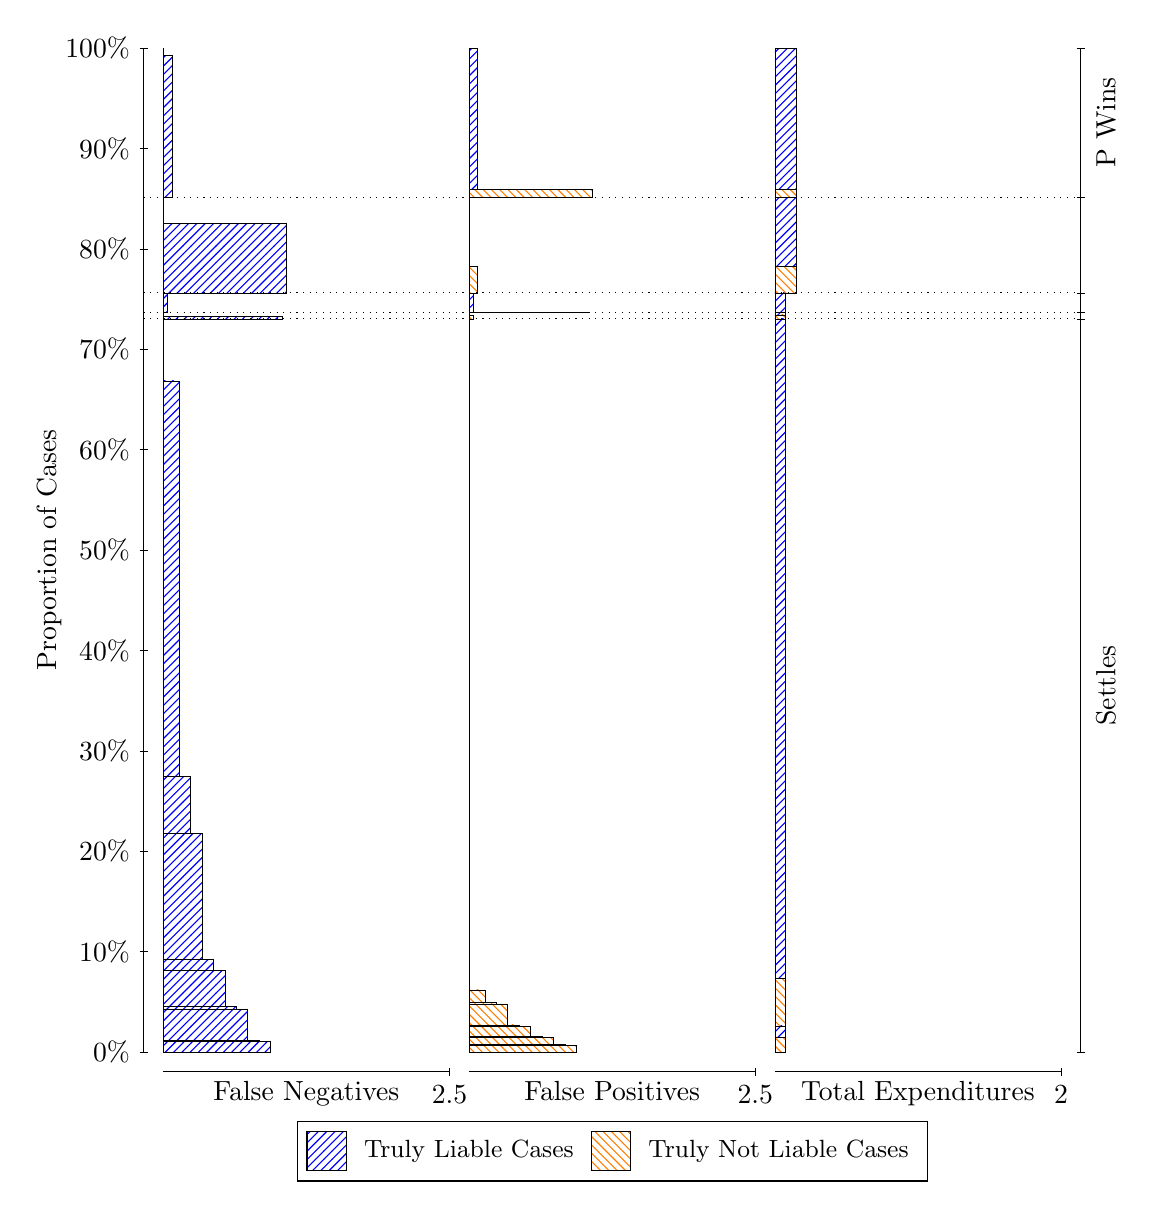
\begin{tikzpicture}
\draw[black, very thin] (1.5,1.75) -- (1.5,14.5);
\node[rotate=90, text=black, anchor=center] at (0.3, 8.125) {Proportion of Cases};
\draw[black, very thin] (1.45,1.75) -- (1.55,1.75);
\node[text=black, anchor=east] at (1.45, 1.75) {0\%};
\draw[black, very thin] (1.45,3.025) -- (1.55,3.025);
\node[text=black, anchor=east] at (1.45, 3.025) {10\%};
\draw[black, very thin] (1.45,4.3) -- (1.55,4.3);
\node[text=black, anchor=east] at (1.45, 4.3) {20\%};
\draw[black, very thin] (1.45,5.575) -- (1.55,5.575);
\node[text=black, anchor=east] at (1.45, 5.575) {30\%};
\draw[black, very thin] (1.45,6.85) -- (1.55,6.85);
\node[text=black, anchor=east] at (1.45, 6.85) {40\%};
\draw[black, very thin] (1.45,8.125) -- (1.55,8.125);
\node[text=black, anchor=east] at (1.45, 8.125) {50\%};
\draw[black, very thin] (1.45,9.4) -- (1.55,9.4);
\node[text=black, anchor=east] at (1.45, 9.4) {60\%};
\draw[black, very thin] (1.45,10.675) -- (1.55,10.675);
\node[text=black, anchor=east] at (1.45, 10.675) {70\%};
\draw[black, very thin] (1.45,11.95) -- (1.55,11.95);
\node[text=black, anchor=east] at (1.45, 11.95) {80\%};
\draw[black, very thin] (1.45,13.225) -- (1.55,13.225);
\node[text=black, anchor=east] at (1.45, 13.225) {90\%};
\draw[black, very thin] (1.45,14.5) -- (1.55,14.5);
\node[text=black, anchor=east] at (1.45, 14.5) {100\%};

\draw[black, very thin] (13.4,1.75) -- (13.4,14.5);
\draw[black, very thin] (13.35,1.75) -- (13.45,1.75);
\node[anchor=west] at (13.35, 1.75) {};
\draw[black, very thin] (13.35,11.061) -- (13.45,11.061);
\node[anchor=west] at (13.35, 11.061) {};
\draw[black, very thin] (13.35,11.141) -- (13.45,11.141);
\node[anchor=west] at (13.35, 11.141) {};
\draw[black, very thin] (13.35,11.39) -- (13.45,11.39);
\node[anchor=west] at (13.35, 11.39) {};
\draw[black, very thin] (13.35,12.604) -- (13.45,12.604);
\node[anchor=west] at (13.35, 12.604) {};
\draw[black, very thin] (13.35,14.5) -- (13.45,14.5);
\node[anchor=west] at (13.35, 14.5) {};

\draw[black, very thin, pattern color=blue, pattern=north east lines] (1.75,1.75) rectangle (3.1125,1.8802);
\draw[black, very thin, pattern color=blue, pattern=north east lines] (1.75,1.8802) rectangle (2.9672,1.8989);
\draw[black, very thin, pattern color=blue, pattern=north east lines] (1.75,1.8989) rectangle (2.8218,2.2875);
\draw[black, very thin, pattern color=blue, pattern=north east lines] (1.75,2.2875) rectangle (2.6765,2.3285);
\draw[black, very thin, pattern color=blue, pattern=north east lines] (1.75,2.3285) rectangle (2.5312,2.7845);
\draw[black, very thin, pattern color=blue, pattern=north east lines] (1.75,2.7845) rectangle (2.3858,2.923);
\draw[black, very thin, pattern color=blue, pattern=north east lines] (1.75,2.923) rectangle (2.2405,4.5237);
\draw[black, very thin, pattern color=blue, pattern=north east lines] (1.75,4.5237) rectangle (2.0952,5.2459);
\draw[black, very thin, pattern color=blue, pattern=north east lines] (1.75,5.2459) rectangle (1.9498,10.272);
\draw[black, very thin, pattern color=orange, pattern=north west lines] (1.75,10.272) rectangle (1.75,11.061);
\draw[black, very thin, pattern color=blue, pattern=north east lines] (1.75,11.061) rectangle (3.2578,11.092);
\draw[black, very thin, pattern color=orange, pattern=north west lines] (1.75,11.092) rectangle (1.75,11.141);
\draw[black, very thin, pattern color=blue, pattern=north east lines] (1.75,11.141) rectangle (1.8045,11.387);
\draw[black, very thin, pattern color=orange, pattern=north west lines] (1.75,11.387) rectangle (1.75,11.39);
\draw[black, very thin, pattern color=blue, pattern=north east lines] (1.75,11.39) rectangle (3.3123,12.269);
\draw[black, very thin, pattern color=orange, pattern=north west lines] (1.75,12.269) rectangle (1.75,12.604);
\draw[black, very thin, pattern color=blue, pattern=north east lines] (1.75,12.604) rectangle (1.859,14.403);
\draw[black, very thin, pattern color=orange, pattern=north west lines] (1.75,14.403) rectangle (1.75,14.5);
\draw[black, very thin, pattern color=orange, pattern=north west lines] (5.6333,1.75) rectangle (6.9958,1.8325);
\draw[black, very thin, pattern color=orange, pattern=north west lines] (5.6333,1.8325) rectangle (6.8505,1.844);
\draw[black, very thin, pattern color=orange, pattern=north west lines] (5.6333,1.844) rectangle (6.7052,1.9388);
\draw[black, very thin, pattern color=orange, pattern=north west lines] (5.6333,1.9388) rectangle (6.5598,1.9524);
\draw[black, very thin, pattern color=orange, pattern=north west lines] (5.6333,1.9524) rectangle (6.4145,2.077);
\draw[black, very thin, pattern color=orange, pattern=north west lines] (5.6333,2.077) rectangle (6.2692,2.095);
\draw[black, very thin, pattern color=orange, pattern=north west lines] (5.6333,2.095) rectangle (6.1238,2.357);
\draw[black, very thin, pattern color=orange, pattern=north west lines] (5.6333,2.357) rectangle (5.9785,2.3762);
\draw[black, very thin, pattern color=orange, pattern=north west lines] (5.6333,2.3762) rectangle (5.8332,2.5398);
\draw[black, very thin, pattern color=blue, pattern=north east lines] (5.6333,2.5398) rectangle (5.6333,11.061);
\draw[black, very thin, pattern color=orange, pattern=north west lines] (5.6333,11.061) rectangle (5.6878,11.111);
\draw[black, very thin, pattern color=blue, pattern=north east lines] (5.6333,11.111) rectangle (5.6333,11.141);
\draw[black, very thin, pattern color=orange, pattern=north west lines] (5.6333,11.141) rectangle (7.1412,11.144);
\draw[black, very thin, pattern color=blue, pattern=north east lines] (5.6333,11.144) rectangle (5.6878,11.39);
\draw[black, very thin, pattern color=orange, pattern=north west lines] (5.6333,11.39) rectangle (5.7423,11.725);
\draw[black, very thin, pattern color=blue, pattern=north east lines] (5.6333,11.725) rectangle (5.6333,12.604);
\draw[black, very thin, pattern color=orange, pattern=north west lines] (5.6333,12.604) rectangle (7.1957,12.701);
\draw[black, very thin, pattern color=blue, pattern=north east lines] (5.6333,12.701) rectangle (5.7423,14.5);
\draw[black, very thin, pattern color=orange, pattern=north west lines] (9.5167,1.75) rectangle (9.6529,1.9328);
\draw[black, very thin, pattern color=blue, pattern=north east lines] (9.5167,1.9328) rectangle (9.6529,2.0817);
\draw[black, very thin, pattern color=orange, pattern=north west lines] (9.5167,2.0817) rectangle (9.6529,2.6887);
\draw[black, very thin, pattern color=blue, pattern=north east lines] (9.5167,2.6887) rectangle (9.6529,11.061);
\draw[black, very thin, pattern color=orange, pattern=north west lines] (9.5167,11.061) rectangle (9.6529,11.111);
\draw[black, very thin, pattern color=blue, pattern=north east lines] (9.5167,11.111) rectangle (9.6529,11.141);
\draw[black, very thin, pattern color=orange, pattern=north west lines] (9.5167,11.141) rectangle (9.6529,11.144);
\draw[black, very thin, pattern color=blue, pattern=north east lines] (9.5167,11.144) rectangle (9.6529,11.39);
\draw[black, very thin, pattern color=orange, pattern=north west lines] (9.5167,11.39) rectangle (9.7892,11.725);
\draw[black, very thin, pattern color=blue, pattern=north east lines] (9.5167,11.725) rectangle (9.7892,12.604);
\draw[black, very thin, pattern color=orange, pattern=north west lines] (9.5167,12.604) rectangle (9.7892,12.701);
\draw[black, very thin, pattern color=blue, pattern=north east lines] (9.5167,12.701) rectangle (9.7892,14.5);
\draw[black, dotted] (1.5,11.061) -- (13.4,11.061);
\draw[black, dotted] (1.5,11.141) -- (13.4,11.141);
\draw[black, dotted] (1.5,11.39) -- (13.4,11.39);
\draw[black, dotted] (1.5,12.604) -- (13.4,12.604);
\draw[black, very thin] (1.75,1.5) -- (5.3833,1.5);
\node[text=black, anchor=north] at (3.5667, 1.5) {False Negatives};
\draw[black, very thin] (5.3833,1.45) -- (5.3833,1.55);
\node[text=black, anchor=north] at (5.3833, 1.45) {2.5};

\draw[black, very thin] (5.6333,1.5) -- (9.2667,1.5);
\node[text=black, anchor=north] at (7.45, 1.5) {False Positives};
\draw[black, very thin] (9.2667,1.45) -- (9.2667,1.55);
\node[text=black, anchor=north] at (9.2667, 1.45) {2.5};

\draw[black, very thin] (9.5167,1.5) -- (13.15,1.5);
\node[text=black, anchor=north] at (11.333, 1.5) {Total Expenditures};
\draw[black, very thin] (13.15,1.45) -- (13.15,1.55);
\node[text=black, anchor=north] at (13.15, 1.45) {2};

\node[text=black, centered, rotate=90] at (13.72, 6.4057) {Settles};



\node[text=black, centered, rotate=90] at (13.72, 13.552) {P Wins};

\draw (7.449999999999999,1.5) node[draw=none] (baseCoordinate) {};
\begin{scope}[align=center]
        \matrix[scale=0.5, draw=black, below=0.5cm of baseCoordinate, nodes={draw}, column sep=0.1cm]{
            \node[rectangle, draw, minimum width=0.5cm, minimum height=0.5cm, pattern color=blue, pattern=north east lines] {}; &
            \node[draw=none, font=\small, text=black] (B) {Truly Liable Cases}; &
            \node[rectangle, draw, minimum width=0.5cm, minimum height=0.5cm, pattern color=orange, pattern=north west lines] {}; &
            \node[draw=none, font=\small, text=black] (B) {Truly Not Liable Cases}; \\
            };
\end{scope}

\end{tikzpicture}
\end{document}